\section{Perturbations in operational orbit}
The perturbations acting on the spacecraft in its orbit around Earth are at first considered separately, analyzing the short (one orbit period) and long period (one year) effects, starting from the arrival orbit after the interplanetary transfer from Venus.
The following perturbations are considered:
\begin{description}
\item [Atmospheric drag]
\begin{equation}
\mathbf{f_d}=-\dfrac{1}{2} \rho v^2 \dfrac{A C_d}{m} \mathbf{\hat v}
\end{equation}
The drag force is directed along the velocity vector $\mathbf {\hat v}$, in opposite direction.
An exponential model, based on the provided scale height, is considered to compute the atmospheric density.
\[
\rho(z)=\rho_0 \exp{\left (-\dfrac{z}{H}\right )}
\]
\item[Solar pressure]
\begin{equation}
\mathbf{f_{sp}} = -\dfrac{W_s}{c} \dfrac{(1+\varepsilon) A}{m} \mathbf{\hat r}_{sun-s/c}
\end{equation}
$c$ is the speed of light in vacuum $c=299792.458$ km/s.

The solar pressure is acting along the direction of the axis between the sun and the spacecraft.

\item[Non uniform mass distribution]

\begin{align}
\mathbf{f_t}&=-\dfrac{3}{2} J_2 \mu \dfrac{R_{\oplus}^2}{r^4} [ 1 - 3\sin^2i\sin^2(\theta+\omega)]\\
\mathbf{f_{\theta}}&=-3 J_2 \mu \dfrac{R_{\oplus}^2}{r^4}\sin^2i\sin(\theta+\omega)\cos(\theta+\omega)\\
\mathbf{f_h}&=-3 J_2 \mu \dfrac{R_{\oplus}^2}{r^4}\sin i \cos i \sin(\theta+\omega)
\end{align}

Only the first zonal harmonic $J_2$ is considered.
\item[Third body effect]
\begin{equation}
\mathbf{f_{tb}}=-\dfrac{\mu_{sun}}{r_{sun-s/c}^2}\mathbf{\hat r}_{sun-s/c}-\dfrac{\mu_{moon}}{r_{moon-s/c}^2}\mathbf{\hat r}_{moon-s/c}
\end{equation}
The gravitational attraction of the Sun and Moon is considered to act as a perturbing acceleration on the spacecraft. 
\end{description}

\subsection{Short period analysis}
The short period analysis considers the perturbations separately acting on the spacecraft, for a period of the orbit. We notice that the drag effect is negligible, since the orbit height varies from $\sim$2800 km to $\sim$5200 km, altitudes where the atmosphere is not present.

\begin{figure}[htp]
\centering
\includegraphics[width=\textwidth]{drag}
\caption{Short period perturbations due to atmospheric drag}
\end{figure}

\begin{figure}[htp]
\centering
\includegraphics[width=\textwidth]{solar}
\caption{Short period perturbations due to solar pressure}
\end{figure}

\begin{figure}[htp]
\centering
\includegraphics[width=\textwidth]{tb}
\caption{Short period perturbations due to third body presence (Sun $\&$ Moon)}
\label{SP3B}
\end{figure}

\begin{figure}[htp]
\centering
\includegraphics[width=\textwidth]{zonal}
\caption{Short period perturbations due to first zonal harmonic J2}
\end{figure}

As shown in fig.\ref{SP3B} the third body effects are particularly perceived on semimajor axis and eccentricity compared to the effects of the others disturbances, instead, zonal harmonics affect, as expected, the right ascension of ascending node and pericenter anomaly. The major effects of disturbaneces are better appreciated into long period analysis as following.

\newpage
\subsection{Long period analysis}
Long period analysis is performed considering the perturbations acting separately and then all together, for a period equal to one terrestrial solar year (365 days). 

\begin{figure}[htp]
\centering
\includegraphics[width=\textwidth]{dragLP}
\caption{Long period perturbations due to atmospheric drag}
\end{figure}

\begin{figure}[htp]
\centering
\includegraphics[width=\textwidth]{solarLP}
\caption{Long period perturbations due to solar pressure}
\end{figure}

\begin{figure}[p]
\centering
\includegraphics[width=\textwidth]{tbLP}
\caption{Long period perturbations due to third body presence (Sun $\&$ Moon)}
\label{tbSP}
\end{figure}

\begin{figure}[htp]
\centering
\includegraphics[width=\textwidth]{zonalLP}
\caption{Long period perturbations due to first zonal harmonic J2}
\end{figure}

\begin{figure}[hth]
\centering
\includegraphics[width=\textwidth]{globalLP}
\caption{Long period perturbations due to overall disturbances}
\label{global}
\end{figure}

On a one year period, two different perturbations affect considerably the spacecraft orbits parameters. Semimajor axis, eccentricity and inclination are particularly affected by third body effects, right ascension and pericenter anomaly are particularly affected by zonal harmonic J$_2$.

As shown in fig.\ref{tbSP} the orbital motion of the Moon affect considerably the eccentricity of the orbits, in fact, it is possible to see how the major variation has a period comparable to the revolution period of the Moon around Earth. The Sun affects the semimajor axis dimension, instead, the combined effects of the Sun and Moon are particularly appreciable on the inclination parameter as depicted in the last image of the fig.\ref{tbSP}.

As regards J$_2$ zonal perturbation it is possible to compare the numerical solution with the analytic ones \cite{mengali} of the pericenter anomaly and right ascension, computed as
\begin{equation}
\bar{\omega}=\omega_0+\frac{3}{2}J_2\bar{n}\left(\frac{R_{\oplus}}{p}\right)^2(2-\frac{5}{2}\sin^2{i})(t-t_0)
\label{OManal}
\end{equation}
and
\begin{equation}
\bar{\Omega}=\Omega_0-\frac{3}{2}J_2\bar{n}\left(\frac{R_{\oplus}}{p}\right)^2\cos{i}(t-t_0)
\label{omanal}
\end{equation}
where
\[
\bar{n}=n\left[1+\frac{3}{2}J_2\left(\frac{R_{\oplus}}{p}\right)^2\sqrt{1-e^2}\left(1-\frac{3}{2}\sin^2{i}\right)\right]
\]
and
\[
n=\sqrt{\frac{\mu}{a^3}}
\]
The overlapping of the numerical solutions and numerical ones is depicted in figures \ref{OM_LP} and \ref{omLP1} respectively for right ascension variations and pericenter anomaly variations.

\begin{figure}[htp]
\centering
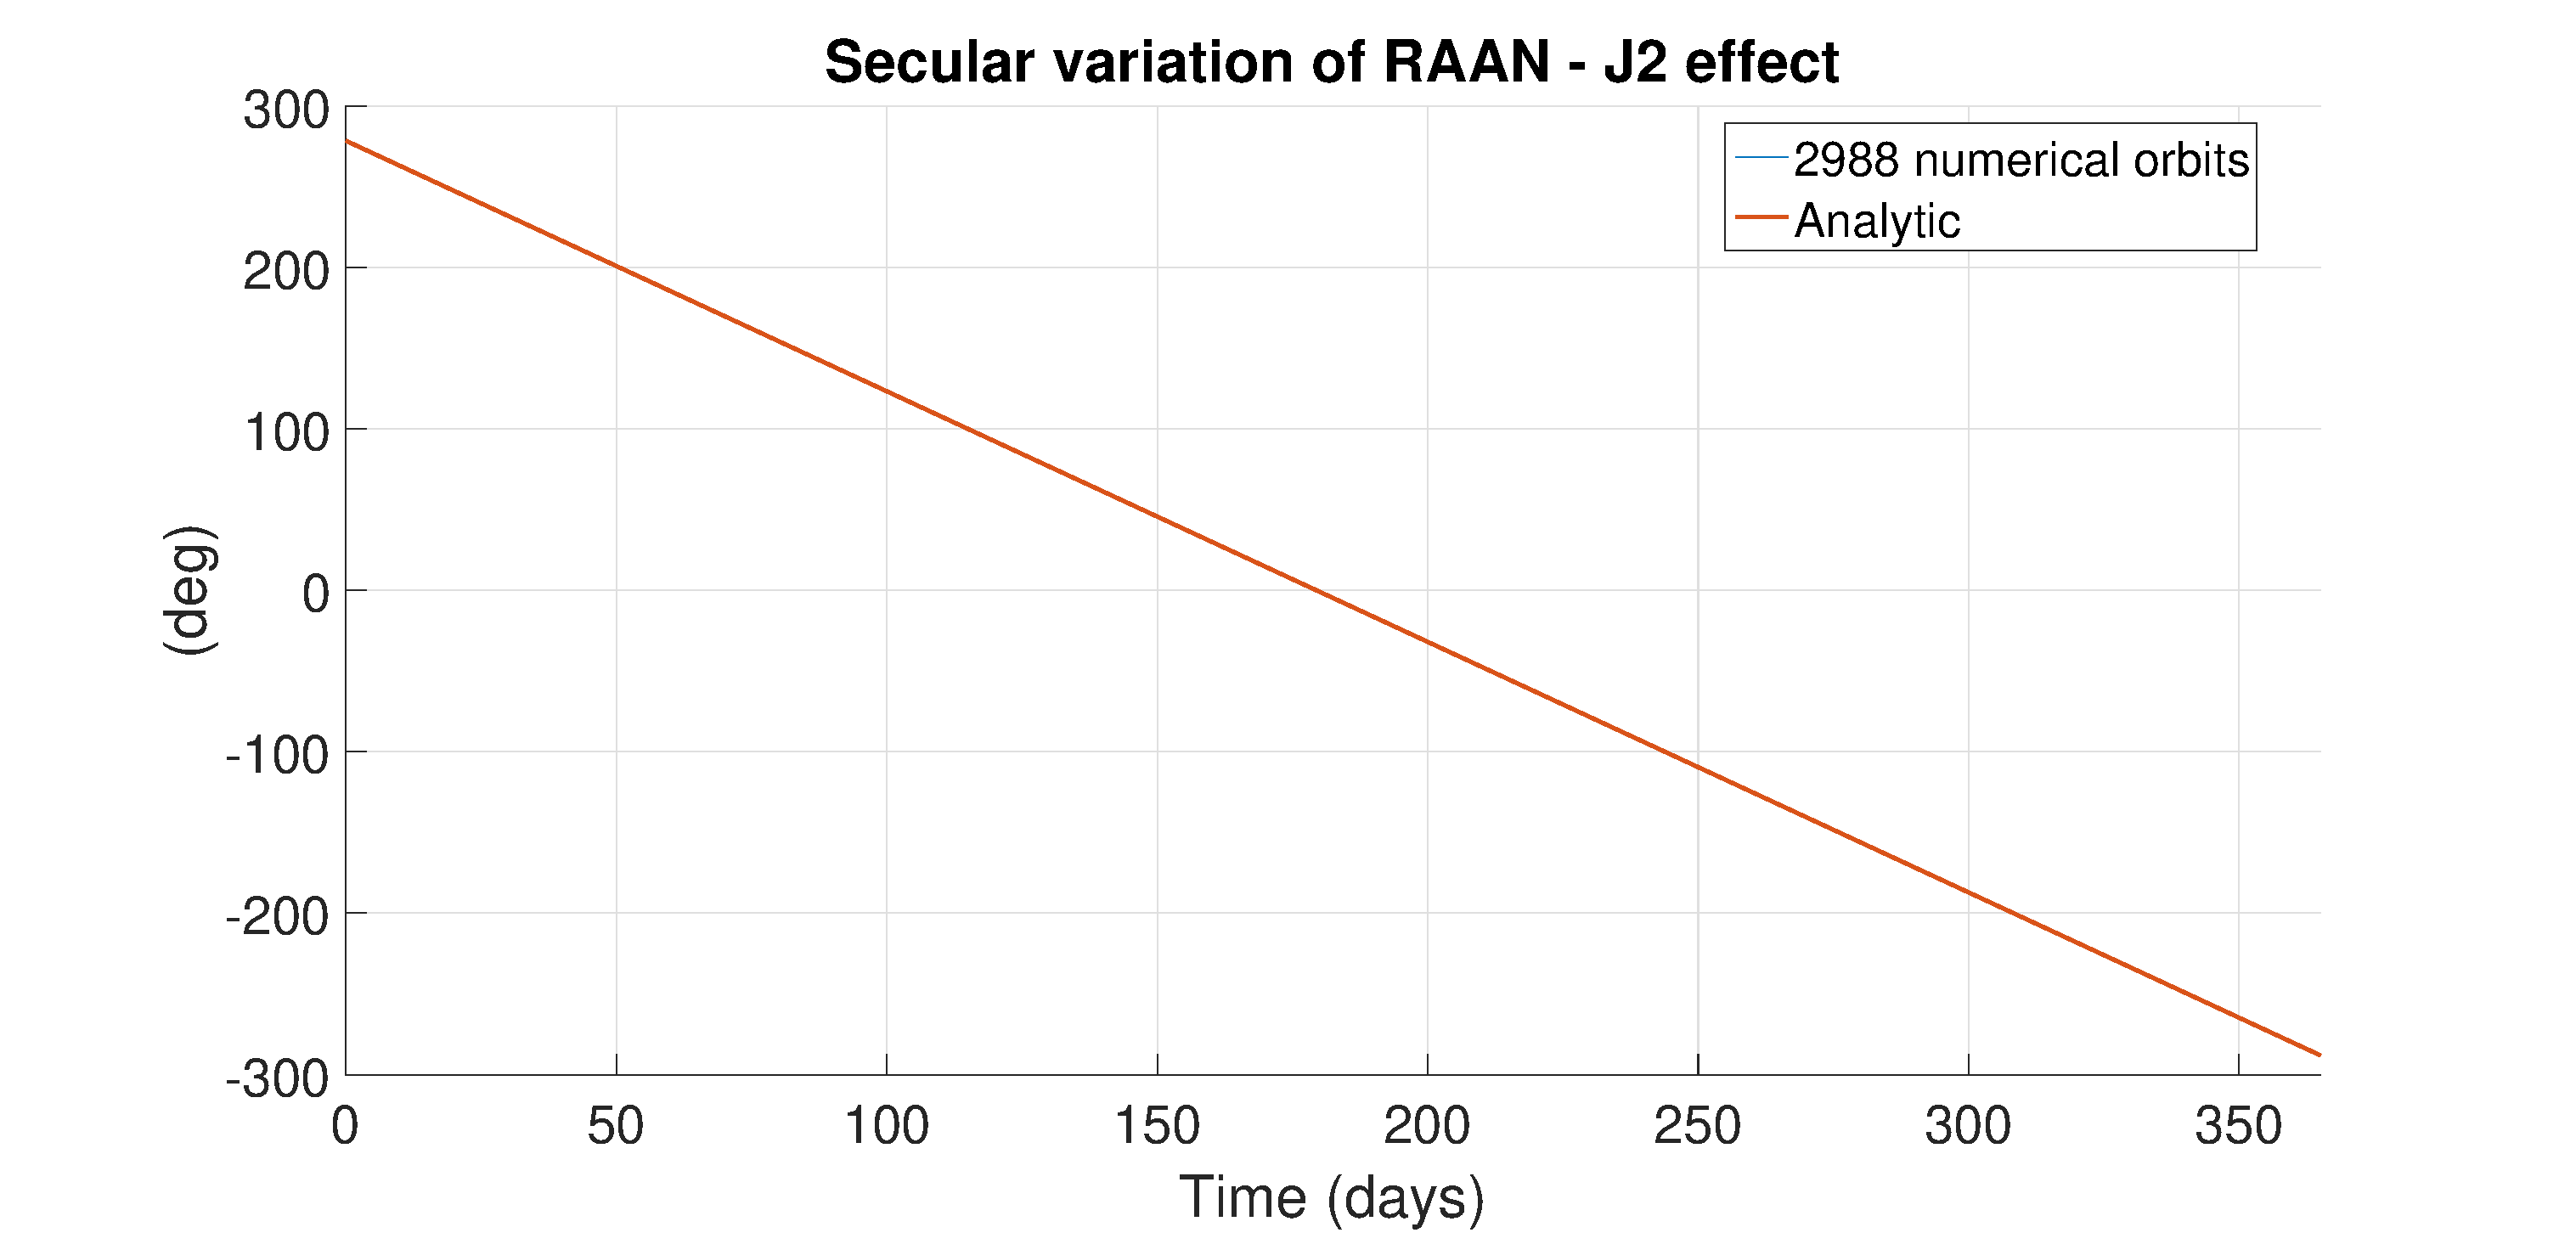
\includegraphics[width=\textwidth]{OM_LP}
\caption{Numerical and analytical variations of $\Omega$ due to first zonal harmonic J2}
\label{OM_LP}
\end{figure}

\begin{figure}[hth]
\centering
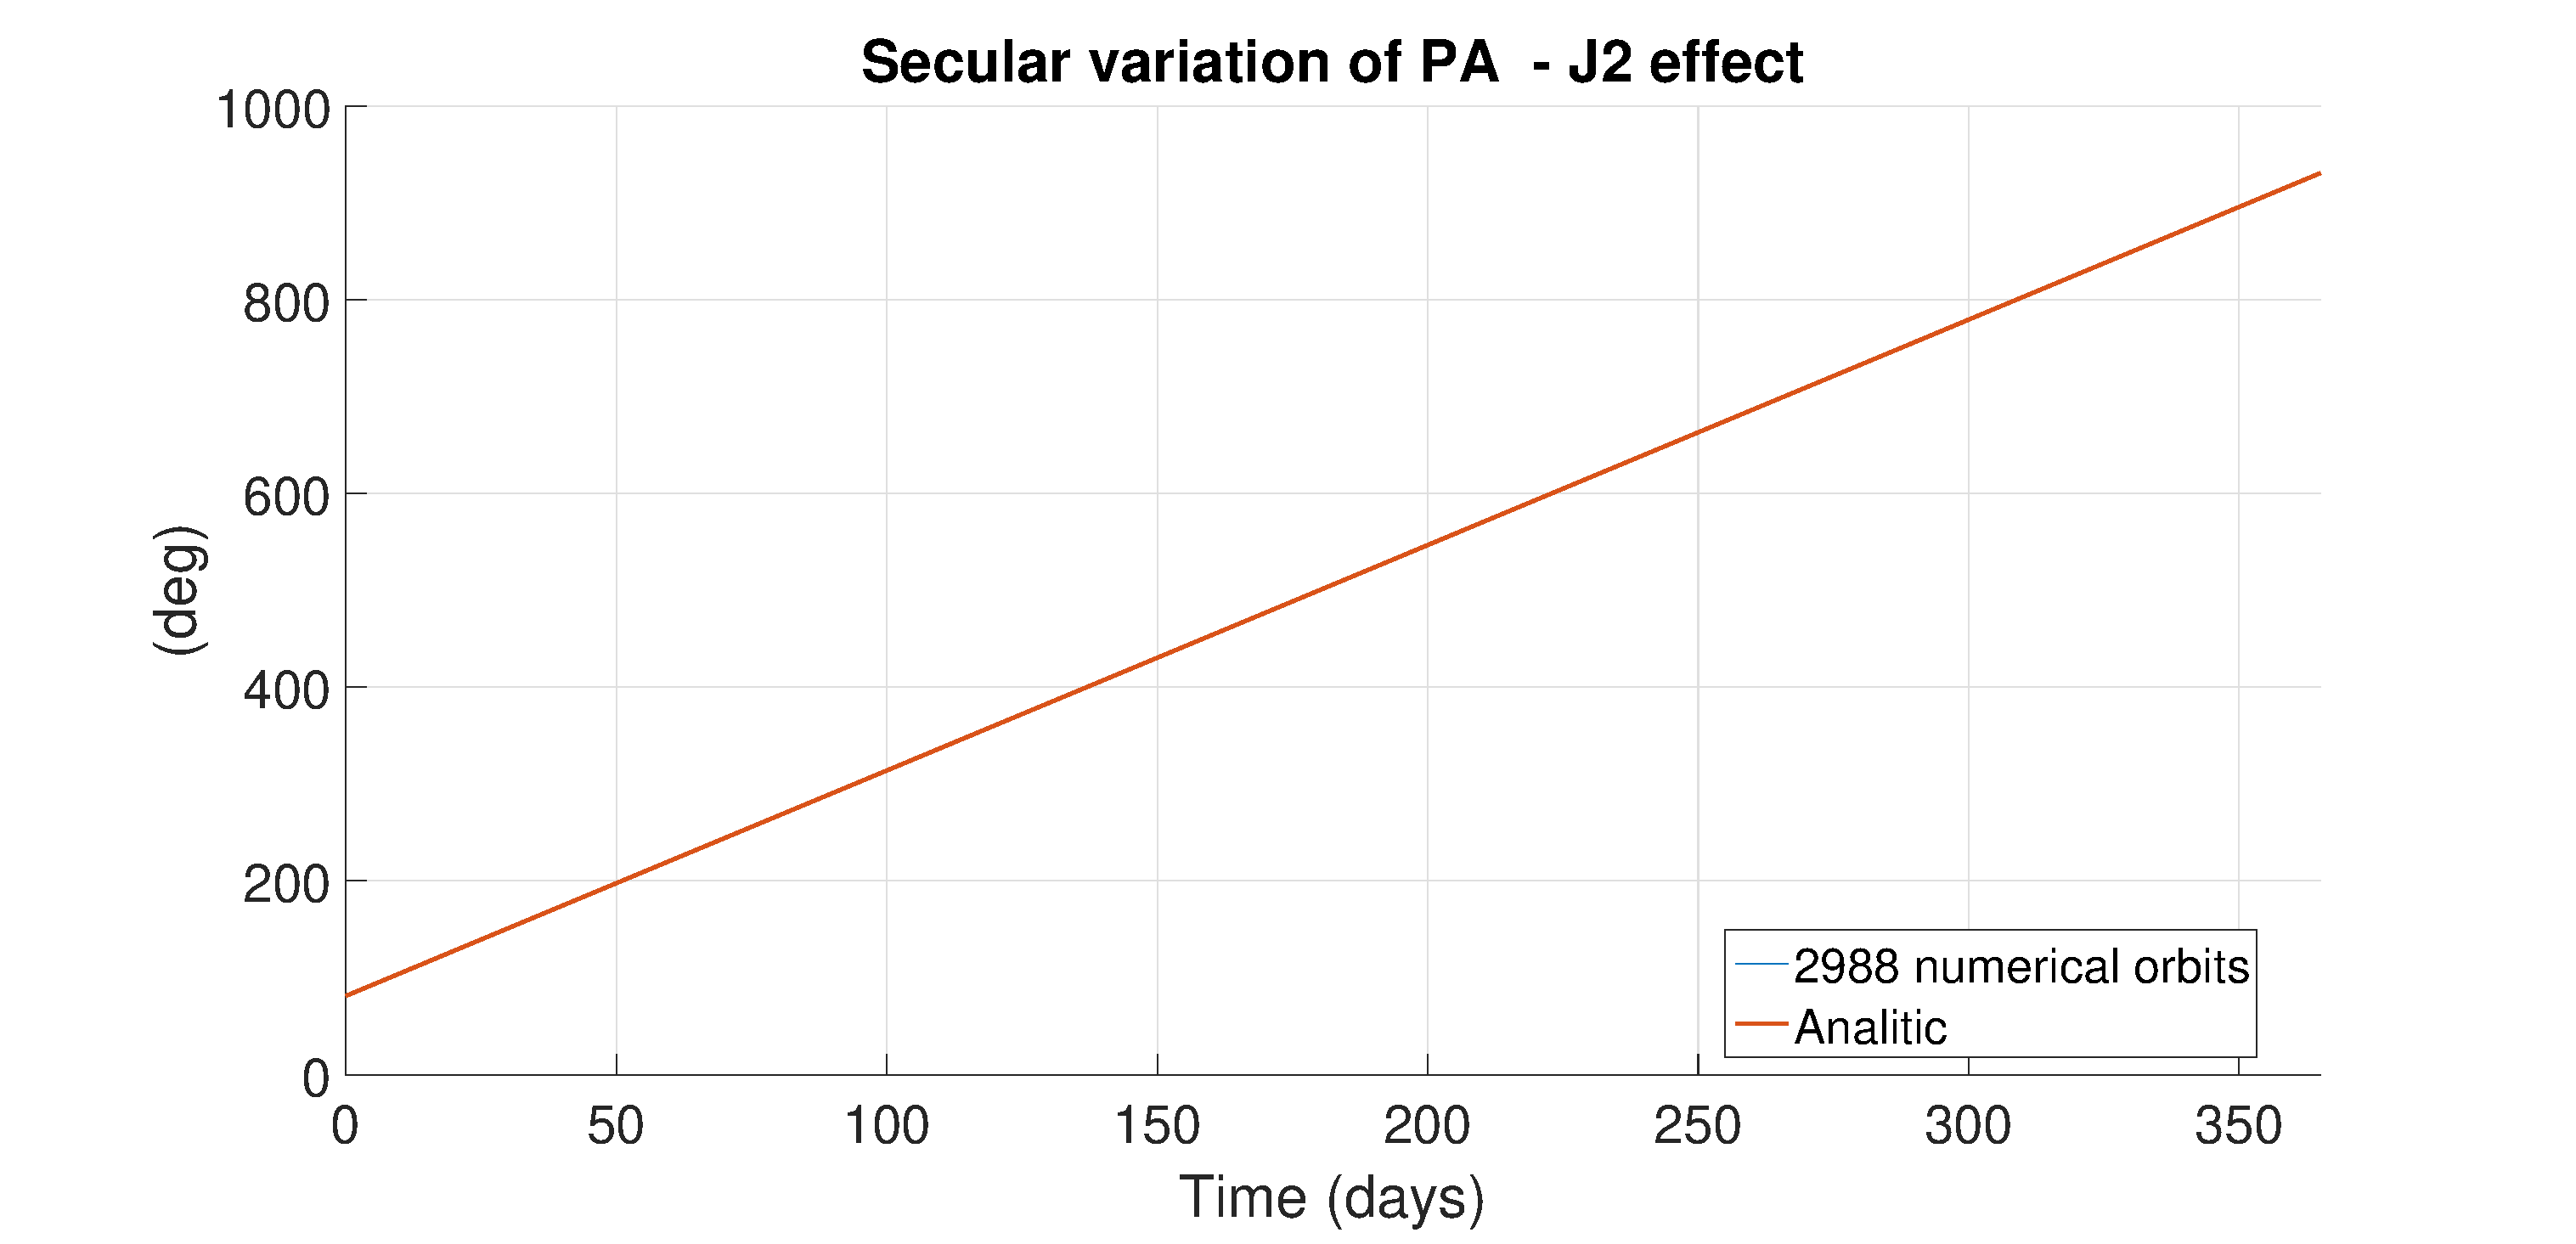
\includegraphics[width=\textwidth]{omLP}
\caption{Numerical and analytical variations of $\omega$ due to first zonal harmonic J2}
\label{omLP1}
\end{figure}

It is easy to understand how the zonal harmonic $J_2$ strongly affects on long period the spacecraft orbits. It is possible to compute the analytic average angular velocity of the nodal axis rotation throughout the one year Earth mission. From equation \ref{OManal} the nodal axis rotation velocity is
\begin{equation}
\dot{\Omega}=-\frac{3\bar{n}J_2R_{\oplus}^2\cos{i}}{2a^2(1-e^2)^2} = -3.13e-7\frac{rad}{s} \simeq -1.55\frac{deg}{day}
\label{OM1}
\end{equation}
Instead, as regards the pericenter anomaly variation, from equation \ref{omanal},
\begin{equation}
\dot{\omega}=\frac{3\bar{n}J_2R_{\oplus}^2(4-5\sin^2{i})}{4a^2(1-e^2)^2}=4.7e-7\frac{rad}{s}\simeq2.33\frac{deg}{day}
\label{om1}
\end{equation}
As seen in fig.\ref{OM_LP} and fig.\ref{omLP1} analytic and numerical behavior are almost perfectly overlapped. Analytic assumption yields to consider the nodal axis rotation angular velocity and pericenter anomaly deviation velocity computed with equations \ref{OM1} and \ref{om1} as a good approximation of actual angular velocities on a long period.